\chapter{Estado del Arte}
En este capítulo se expresará cómo ha sido la evolución histórica de las principales herramientas a desarrollar durante el proyecto así como las diferentes alternativas más importantes dentro de cada campo.   

\section{Asistentes Virtuales}

\subsection{Historia de los Chatbots}

Un chatbot es una aplicación de software capaz de mantener una conversación con un usuario dando una serie de respuestas automáticas, establecidas con anterioridad a diferentes entradas que pueda dar el usuario. Existen distintas teorías sobre el origen de los chatbots. 

La primera de ellas, defiende que en la década de 1950, el matemático inglés Alan Turing investigó si una máquina sería capaz de imitar las respuestas de un humano mediante el análisis de una conversación de texto entre un humano y una máquina. 

La segunda, más extendida, sitúa el origen en el año 1966 en el Instituto Tecnológico de Massachusetts (MIT), allí el profesor de informática Joseph Weizenbaum desarrolló en el laboratorio de inteligencia artificial el programa \textit{Eliza}, el concepto es que actuara como si se tratase de un terapeuta. Funcionaba de la siguiente manera: examinaba palabras clave que tenía el enunciado del emisor para poder responder con una serie de oraciones que tenía previamente registradas.

En 1972, surgió el chatbot \textit{Parry}, que simulaba ser una persona con esquizofrenia paranoide. A diferencia de Eliza disponía de una estrategia de comunicación cimentada en premisas y ''respuestas emocionales'' en base a las interacciones con los usuarios. \cite{StreamGenerator}

Como detalle curioso, Eliza y Parry fueron puestos a conversar entre sí mediante la red ARPANET \footnote{ARPANET: red de ordenadores creada por el Departamento de Defensa de los Estados Unidos para conectar varias instituciones académicas y estatales.}  
Posteriormente fue desarrollado \textit{Jabberwacky} por el programador inglés Rollo Carpenter, capaz de mantener una conversación mediante la voz. Aunque fue terminado en 1981 no fue hasta 1997 cuando fue publicado online.
A partir del año 2006 han surgido una gran cantidad de chatbots entre los que cabe destacar:

IBM Watson, nombrado así por el primer director ejecutivo de IBM. En un principio fue desarrollado para responder preguntas y respuestas ideadas por humanos para el concurso Jeopardy. El concurso es el típico de preguntas y respuestas solo que las preguntas son formuladas mediante juegos de palabras y giros lingüisticos. Se presentó al concurso en 2011 por primera vez y fue capaz de ganar a dos especialistas. A partir de ese instante, ha pasado por varias adaptaciones utilizando procesamiento de lenguaje natural y machine learning\footnote{Machine Learning: disciplina dentro de la Inteligencia Artificial que crea sistemas y software capaces de aprender automáticamente} para procesar una gran cantidad de datos. En 2013, IBM anunció que Watson podía ser utilizado para la toma de decisiones en el tratamiento del cáncer de pulmón. 

Tal vez el chatbot más conocido mundialmente sea el asistente virtual desarrollado por Apple, \textit{Siri}. Utiliza consultas dadas mediante comandos de voz para ayudar al usuario de diversas formas, realizar tareas, recordatorios, búsquedas y modificar configuraciones del sistema tal y como se observa en la figura \ref{fig:siri_gui}.

De este mismo estilo tenemos los chatbot \textit{Alexa} creado por Amazon,\textit{Cortana} desarrollado por Microsoft y \textit{Google Now} desarrollado por Google.


\begin{figure}[H]
    \centering
    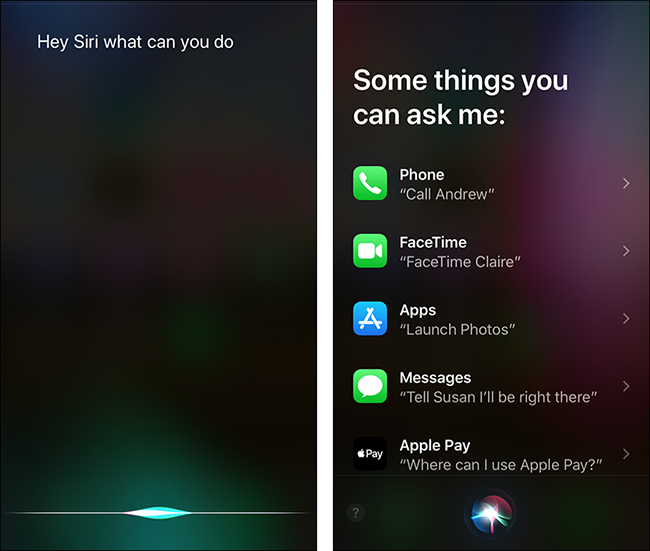
\includegraphics[scale=0.4]{{include/figuras/siri.png}}
    \caption{Interfaz de Siri}
    \label{fig:siri_gui}
\end{figure}

La utilización de estos asistentes ha crecido exponencialmente debido a la necesidad de dar servicios a los clientes, sin importar la hora ni el lugar ya que están siempre disponibles cuando el usuario lo necesite.
Hoy en día se están implementando cada vez más en servicios de mensajería instantánea para la transmisión de noticias, las más destacables son Telegram (figura \ref{fig:telegram}), Slack, Whatsapp, Discord, Skype, Kik y WeChat

\begin{figure}[h]
    \centering
    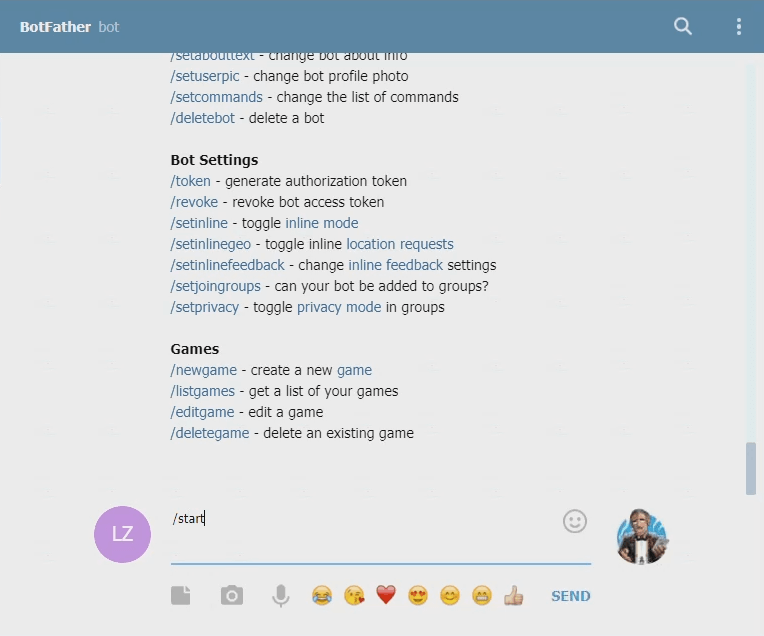
\includegraphics[width=0.5\textwidth]{include/figuras/BotFather.png}
    \caption{Telegram BotFather}
    \label{fig:telegram}
\end{figure}
Alguna de estas aplicaciones han desarrollado servicios mediante los cuales puedes crear nuevos bots sin tener que programar una sola linea de código, como puede ser BotFather de Telegram. Así como tiendas con búsquedas y sistemas de valoraciones para aumentar el uso de estas aplicaciones. 

\subsection{Frameworks de Desarrollo de Chatbots}

Un framework es un tipo de estructura con una serie de archivos y pautas que se utiliza para desarrollar proyectos con una estructura y metodología, es decir, algo así como una plantilla que simplifica la creación de una solución.

\subsubsection{DialogFlow}
Framework de desarrollo de chatbots creado en 2010 y mantenido por Google\cite{Dialogflow}. Es capaz de comprender el lenguaje natural y nos brinda herramientas para la fabricación de diálogos (figura \ref{fig:dialogflow_gui}) y la recreación de conversaciones. Destaca por la gran cantidad de interfaces de conversación en los que se puede desplegar (Google home, google assistant, wereables, teléfonos, coches). Tiene soporte para más de 14 idiomas y es capaz de resolver abreviaturas y funcionar con faltas de ortografía. 
Posee una interfaz muy intuitiva y permite crear chatbots en una cantidad pequeña de tiempo. 

\begin{figure}[H]
    \centering
    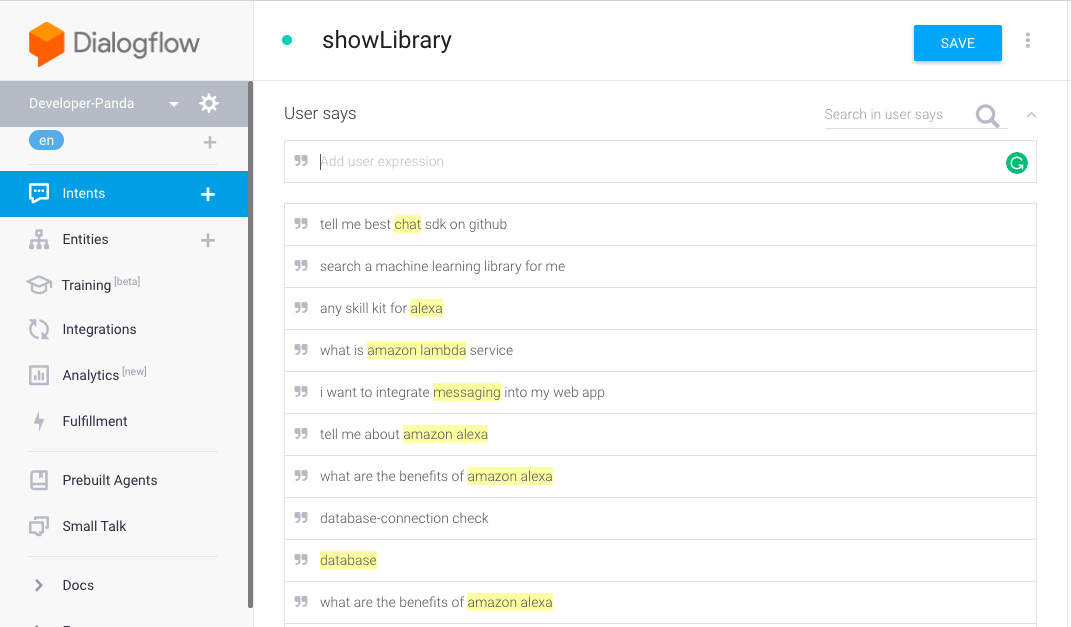
\includegraphics[scale=0.3]{{include/figuras/DialogFlow.png}}
    \caption{Interfaz de dialogflow}
    \label{fig:dialogflow_gui}
\end{figure}


\subsubsection{Microsoft Bot Framework}
Desarrollado por Microsoft, crea chatbots rapidamente a través de la herramienta Microsoft Bot Builder y los conecta con Azure Bot Service, lo que nos permite una rápida creación del bot ya que nos proporciona diversas plantillas para seleccionar cuando se está creando el bot y nos brinda todas las mejoras de la nube creada por Microsoft. Puede editarse con directamente desde la página web usando el editor de Azure o algún IDE de desarrollo como Visual Studio o Visual Studio Code \cite{MicrosoftBotBuilder}. Posee su propio sistema de procesamiento natural del lenguaje llamado LUIS (\textit{Language Understanding Intelligent Service}).  

\subsubsection{IBM Watson}
Creado por IBM, es capaz de comprender y responder a las preguntas de los usuarios mediante lenguaje natural \cite{ibmWatson}. Watson está compuesto actualmente por un clúster de al menos 750 servidores \textit{IBM Power 750}, con unos 16 TB de memoria RAM, lo que proporciona una potencia de cálculo bruto de unos \textbf{80 Petalops}, convirtiéndolo así en uno de los supercomputadores más potentes del mundo. 

\subsubsection{Amazon Lex}
Creado y gestionado por Amazon, permite establecer comuncicaciones con todos sus productos Eco y con su asistente virtual Alexa. Es una de las mejores herramientas en cuanto a conversión de voz a texto. Con esta herramienta se pueden crear bots con un lenguaje natural sofisticado. A diferencia de los anteriores, tiene una interfaz más intuitiva para principiantes aunque por el contrario, dispone de menos herramientas, aunque posee todas las necesarias en un chatbot.

\subsubsection{Rasa}
Por último cabe destacar Rasa, una framework \textit{Open Source} de Machine Learning que nos permite crear conexiones entre las máquinas y el usuario. Posee herramientas para entender al usuario mediante el componente Rasa NLU (Natural Langugage Understanding), generar el diálogo con Rasa NLG (Natural Language Generation) y un motor (Rasa Core) capaz de definir cuál será la siguiente acción a tomar en función del mensaje transmitido por el usuario.   


\subsection{Librerías}

Una librería es uno o varios archivos escritos en algún tipo de lenguaje de programación, que proporcionan varias funcionalidades. Al contrario que un framework, una librería no establece la estructura sobre cómo debe realizarse el desarrollo, sino que da funcionalidades genéricas que han sido programadas con anterioridad y evitan que haya que escribir código de más, aumentando la calidad del código y reduciendo el tiempo de desarrollo.
Vamos a analizar las librerías existentes más importantes para el lenguaje de programación Python, debido a que se trata de un lenguaje simple, elegante ordenado, portable y que requiere de pocas líneas de código para generar programas completos.

\subsubsection{Chatterbot}
Se trata de una librería de Machine Learning basada en las conversaciones y diálogos tradicionales. Está diseñada de manera independiente al idioma, por lo que se puede entrenar en cualquier lenguaje que está asegurado su correcto funcionamiento. 
El Machine Learning implementado en Chatterbot consigue que mediante la interactuación con los humanos permite que mejore su propio conocimiento. También es posible implementarlo junto a otras librerías para añadir funcionalidad como Text to Speech \footnote{Text to Speech: por sus siglas en inglés TTS, procedimiento de síntesis mediante el cual se transforma el texto escrito en voz.}

Es también compatible con librerías para aportar más funcionalidades como puede ser la conversión de texto a voz y así poder interactuar con el usuario sin necesidad de escribir.

\subsubsection{Natural Language ToolKit} NTLK por sus siglas en inglés, se trata de una plataforma para crear chatbots con lenguaje humano. Dispone de funcionalidades muy interesantes desde el punto de vista del reconocimiento del lenguage como la tokenización , derivación, etiquetado, análisis y razonamiento semántico.

\subsubsection{ChatbotAI} Nos permite crear un chatbot con muy pocas líneas de código. Genera un controlador del chat y bots con inteligencia artificial que permiten una integración muy sencilla con API Rest. Esta inteligencia artificial nos genera múltiples características como aprender, memorizar, manejar conversaciones según el tema \cite{chatbotAI}. 

\subsubsection{Tensorflow} Es uan plataforma de código abierto gestionada por Google. Se trata de una biblioteca de aprendizaje automático con la que es posible construir y entrenar redes neuronales para detectar patrones y correlaciones en el aprendizaje y razonamiento de los humanos. Tiene diversas formas de interacción con el usuario (interfaces web, API Rest, interfaces gráficas de usuario, y líneas de comandos).

\subsection{Procesamiento de Lenguaje Natural}
Una de las partes más importantes de un asistente virtual es el Natural Lenguage Processinng (NLP), gracias a esta herramienta, el programa es capaz de entender la forma en la que nos expresamos los humanos. 
El procesamiento del lenguaje natural es una rama de la inteligencia artificial la cual se encarga de analizar y estudiar las interacciones en lenguaje natural entre los humanos y los ordenadores. Este campo posee varias funciones atrayentes.

\begin{itemize}
    \item \textbf{Comprensión del lenguaje natural}: mediante esta función el programa consigue analizar lo que dice el usuario y comprender el mensaje. Para ello es estrictamente necesario que exista una base de datos del lenguaje en el que queremos que se exprese el chatbot de manera que pueda comprender la gramática, la semántica y el vocabulario del lenguaje que queremos que domine.
    \item \textbf{Recuperación de la información}: esta parte es la encargada de extraer las palabras claves del texto proporcionado.
    \item \textbf{Generación del lenguaje natural}: capacidad de dar respuestas a los mensajes enviados en lenguaje natural. Esta parte del programa se encarga de escoger las posibles respuestas y establecer un orden para que la respuesta proporcionada sea la más indicada y correcta gramaticalmente.
    \item \textbf{Reconocimiento y síntesis del lenguaje hablado}: hace que el chatbot sea capaz de transformar las respuestas que se le entregan mediante el habla y transformarlas a texto para su tratamiento. Una vez la respuesta del chatbot se genere, el módulo se encargará de convertirla a voz.
    \item \textbf{Detección de emociones y sentimientos}: hay ciertos programas que a través del estudio del lenguaje de las entradas que da el usuario son capaces de detectar los sentimientos y emociones.
\end{itemize}

\subsection{Ventajas e Inconvenientes de Utilizar Chatbots en un Entorno Profesional}
El afloramiento de los asistentes virtuales ha permitido la mejora y la automatización de procesos y servicios dentro del entorno profesional pero al no tener todas las habilidades que posee un humano, su utilización también posee ciertos inconvenientes.

\subsubsection{Ventajas}

\begin{itemize}
    \item Disponibilidad: un chatbot una vez implementado puede funcionar 24 horas al día 7 días a la semana.
    \item Reducción de costes: puesto que es capaz de responder las preguntas más frecuentes y realizar las tareas más solicitadas no será necesario tener asistentes humanos, permitiendo una reducción de costes y su posible utilización en otros campos más necesarios.
    \item Auto-aprendizaje: posee algún tipo de inteligencia artificial es capaz de aprender nuevos comportamientos a través de las interacciones con los clientes así como nuevos comportamientos que no hayan sido programados. 
    \item Eficiencia: Un asistente humano tiene una capacidad limitada de atención en un rango de tiempo mientras que el asistente puede tener tantas instancias como sea necesario.
\end{itemize}



\subsubsection{Inconvenientes}

\begin{itemize}
    \item Inteligencia: aunque tenga implementado inteligencia artificial, un asistente no es más inteligente que un humano y hay veces que no entiende el mensaje que el usuario le entrega y puede provocar un atasco del proceso. Esto puede llevar a que si el usuario pierde la paciencia, no se complete el proceso de compra.
    \item Tiempo: es necesario emplear tiempo en entrenar al asistente.
    \item Toma de decisiones: un chatbot no es capaz de decidir en base a lo que se haya enseñado con anterioridad.
    \item Coste: es cierto que la implementación de un chatbot permite reducir los costes de mano de obra aunque si bien es cierto que en un primer momento el coste de implementarlo puede ser mayor puesto que hay que programarlo de tal manera que se adapte al campo de la empresa, es decir, hay que especializarlo.
\end{itemize}


\subsection{Principales Aplicaciones de los Chatbots}

\subsubsection{Información}
Durante una crisis sanitaria como la que está viviendo el planeta con el virús SARS-CoV-2 la tendencia más normal es que noticias falsas o bulos se propaguen con una gran velocidad aunque cada día hay más gente que busca información y ayuda a través de recursos en línea. 

Para todos ellos, la Organización Mundial de la Salud (OMS) \cite{oms} ha desarrollado un chatbot para que las personas se mantengan informadas mediante un chatbot implementado en la aplicación de mensajería instantánea WhatsApp, ha sido diseñado de tal manera que permita dar información rápida y fiable sobre temas relacionados con el coronavirus. Se trata de un bot que funciona mediante comandos, utilizando emojis o palabras que nos indica el propio bot nos proporcionará información sobre varios temas como podemos observar en la figura \ref{fig:oms}. De momento el bot sólo esta disponible en inglés aunque está en estudio el ampliarlo a castellano, árabe, chino, francés y ruso.

\begin{figure}[H]
    \centering
    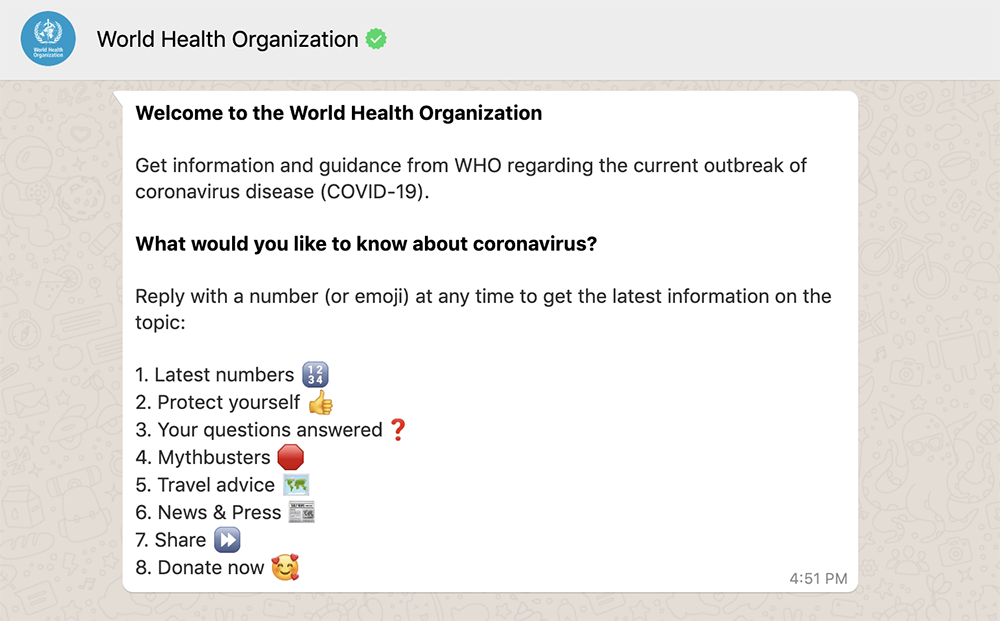
\includegraphics[scale=0.6]{include/figuras/oms.png}
    \caption{Interfaz World Health Organization}
    \label{fig:oms}
\end{figure}

\subsubsection{Salud}
En consecuencia a lo expuesto en la sección anterior, mucha gente en contraindicación de lo que aconsejan los médicos busca información sobre los síntomas que puedan padecer a través de internet. En esta línea se desarrolló Woebot \cite{woebot}, un chatbot que ayuda a reducir los síntomas de la depresión escuchando de forma activa los mensajes que envía el usuario y reaccionando a ellos con ánimo y con GIFs divertidos a mensajes positivos (figura \ref{fig:woebot}). Combina años de investigación en el campo de la psicología con la inteligencia artificial y el procesamiento del lenguaje natural permitiendo que se evalúe el estado emocional del usuario y guiándolo para recibir la ayuda correcta de los profesionales necesarios en el momento adecuado.

\begin{figure}[H]
    \centering
    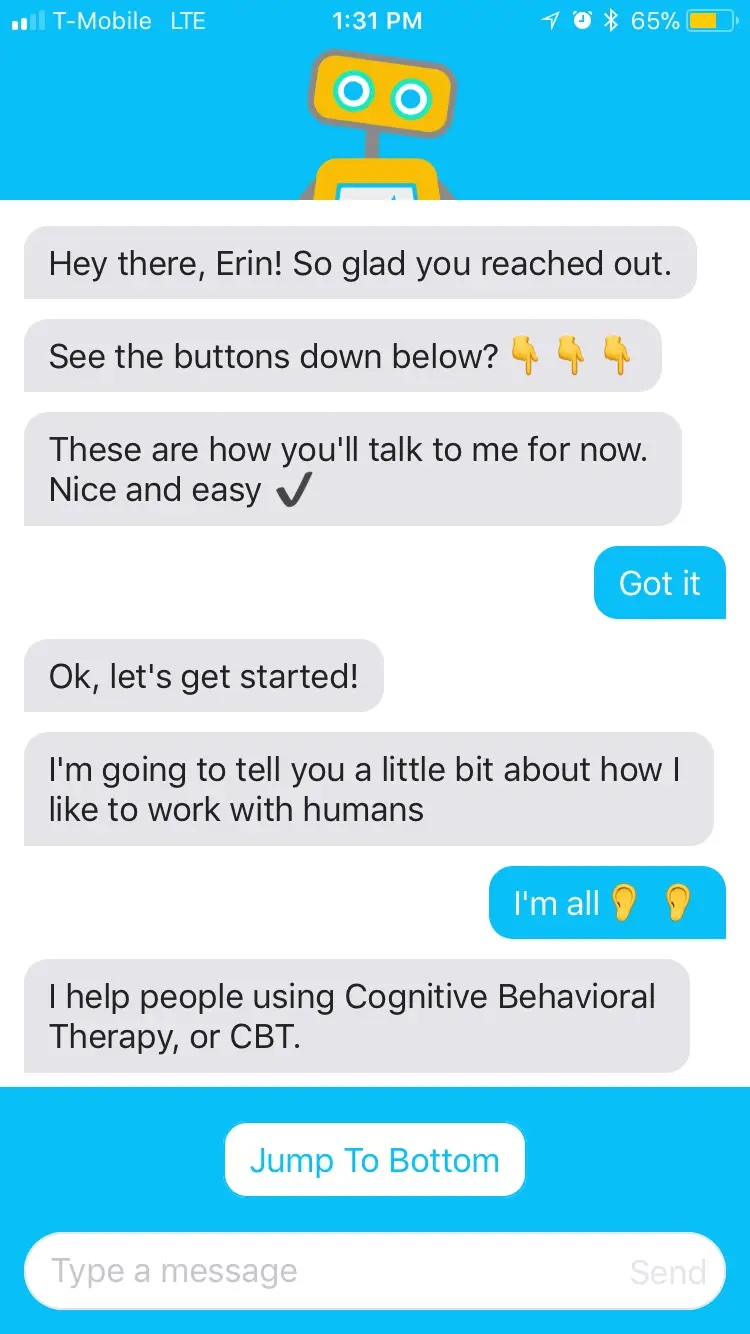
\includegraphics[scale=0.15]{include/figuras/woebot.jpg}
    \caption{Interfaz Woebot}
    \label{fig:woebot}
\end{figure}


\subsubsection{Viajes}
Un bot de viaje puede ahorrar una cantidad significativa de tiempo a los usuarios (organización del viaje, lugares de interés a visitar) además mediante el uso de inteligencia artificial han hecho que varias empresas del sector turísitico se lancen a la implementación de un chatbot que por un lado aumente su número de ventas y por otro reduzca la cantidad de personas necesarias para contestar a todos los usuarios con dudas.
A día de hoy, uno de los mejores chatbots de la industria es el desarrollado por KLM Royal Dutch Airlines \cite{klm}, este chatbot funciona a través de Facebook Messenger, como se puede ver en la figura \ref{fig:klm}, pero con la particularidad que utiliza un complemento de casilla de verificación de Facebook Messenger a la hora de realizar el pago de tal manera que capaz de proporcionar información sobre la tarjeta de embarque, el check-in y actualizaciones del estado del vuelo a través de la aplicación de mensajería instantánea.
Antes de la implementación del chatbot, KLM tenía que contestar unas 15000 conversaciones a la semana a través de las redes sociales en una docena de idiomas distintos, para poder tratar todas estas conversaciones se requiere una gran cantidad de personal y aún así existirán horarios en los cuales no se pueda conversar con el usuario. Para solucionarlo comenzaron a estudiar varias formas para prestar una atención excelente en cualquier momento del día, rápida y personalizada, como resultado llegaron a la conclusión de implementar un chatbot. 
En el primer mes de funcionamiento, el volumen de mensajes en Facebook aumentó un 40 por ciento y envió 1.7 millones de mensajes a más de 500000 clientes.

\begin{figure}[H]
    \centering
    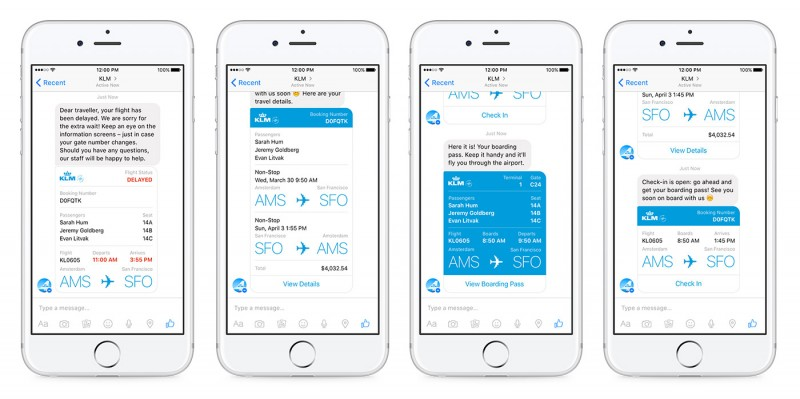
\includegraphics[width=0.8\textwidth]{include/figuras/klm-chatbot.jpg}
    \caption{Interfaz gráfica chatbot KLM}
    \label{fig:klm}
\end{figure}


\subsubsection{Banca}
En los últimos tiempos los bancos están intentando mejorar las relaciones y la comunicación con sus clientes. Este sector tiene fama de utilizar aplicaciones y sistemas arcaicos pero cada vez son mas las entidades que buscan actualizarse y llegar a más clientes. 
El holding bancario Capital One \cite{eno} es uno de los más grandes de Estados Unidos y en 2018 lanzó su chatbot \textit{ENO} (figura \ref{fig:eno}), se trata de un chatbot conversacional, es decir, es capaz de continuar una conversación y no funciona mediante comandos. Los clientes pueden mandar un sms a Eno en cualquier momento a través de la página web, la aplicación móvil del banco para comprobar transacciones recientes, el saldo o incluso para informar sobre algún problema con la tarjeta de crédito. Tiene la capacidad de incluso avisar cuando se cobra de más por una factura.

\begin{figure}[H]
    \centering
    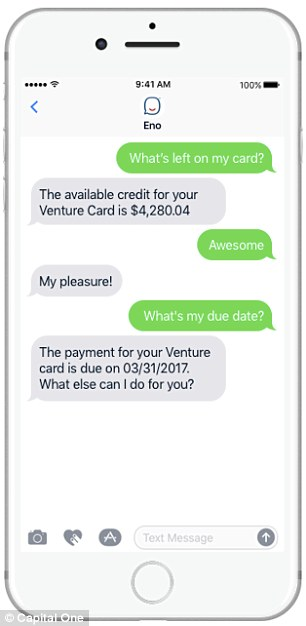
\includegraphics[scale=0.3]{include/figuras/Eno.jpg}
    \caption{Interfaz gráfica Eno}
    \label{fig:eno}
\end{figure}


En España existen algunas alternativas como por ejemplo, la aplicación imaginBank implementado por La Caixa a través de Facebook Messenger.

\subsubsection{Entretenimiento}
Los chatbots también se pueden emplear para realizar planes y lugares de ocio. Un ejemplo de esto es el asistente Mahoudrid creado por la empresa Mahou en colaboración con Ontwice basándose en la guia de ocio de nombre homónimo. 

Este asistente es capaz de recomendar locales, bares, tapas y planes. Es un bot conversacional implementado a través de Facebook Messenger mediante inteligencia artificial y te recomienda el plan perfecto en base a lo que desees tomar y tu estado de ánimo. 

\subsubsection{Restauración}
En la actualidad existen múltiples chatbots que ayudan al usuario a consultar recetas o consejos de dietética, sin embargo, el verdadero potencial de estos es el de poder recomendar restaurantes cercanos a la ubicación del usuario e incluso realizar un pedido simplemente escribiendo en un chat de mensajería instantánea y que lo tengas en tu casa en el menor tiempo posible sin tener que realizar ninguna llamada telefónica. 

Un ejemplo es el chatbot desarrollado por Burguer King \cite{burguer} e implementado en WhatsApp que se muestra en la figura \ref{fig:burguer}.


\begin{figure}[H]
    \centering
    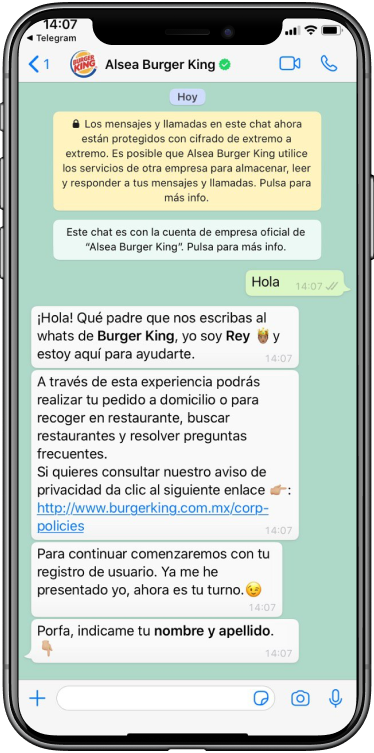
\includegraphics[scale=0.4]{include/figuras/BurguerKing.png}
    \caption{Chatbot Burguer King}
    \label{fig:burguer}
\end{figure}


\section{Bases de Datos}
\subsection{Historia de las bases de datos}

Hay que remontarse un poco atrás en el tiempo, concretamente hasta 1880 cuando Herman Hollerith desarrolló una máquina para procesar los datos más rápido de lo que los humanos podían hacerlo. Desarrolló unas tarjetas perforadas mediante las cuales podía realizar un censo de la población completa de Estados Unidos en solo dos años, algo que en esa época era poco más que una quimera. Aun así, la primera vez que se tiene conocimiento del uso del término bases de datos fue en el año 1963 en un simposio celebrado en California y se refiere a ella como un conjunto de información relacionada y que tiene cierta estructura.

Los primeros modelos que fueron desarrollados fueron bases de datos jerárquicas y en red, pero rápidamente se vio que estaban muy limitadas técnicamente y eran demasiado simples. Posteriormente, IBM revolucionó el sector en la década de los 70 creando el modelo relacional de base de datos, mucho más potente y muy bien adoptada por el mundo laboral.
En los 2000 empezaron a aparecer proyectos de código libre que supusieron una competencia en un sector liderado siempre por sistemas privados (IBM y Oracle), entre los más usados destacan MySQL y PostgreSQL. La tendencia a la utilización de sistemas NoSQL contribuyó al detrimento de los sistemas de bases de datos de las grandes empresas. \cite{sanchez2016historia} 

\subsection{Tipos de Bases de Datos}
\subsubsection{Bases de Datos Jerárquicas}

Se trata del modelo más antiguo, se ha visto superado por el modelo relacional. El lenguaje de marcado XML utiliza este tipo de modelo para almacenar los datos. El sistema más conocido es el IMS/DB creado por IBM.

\begin{figure}[h]
    \centering
    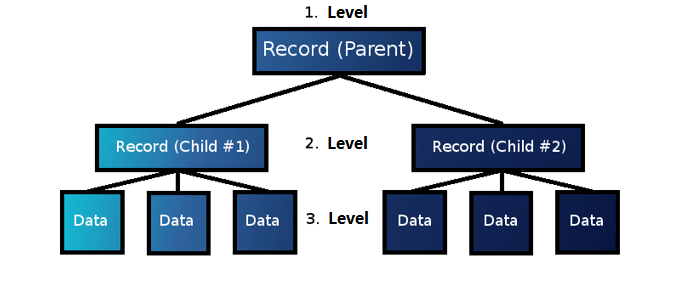
\includegraphics[scale=0.4]{{include/figuras/Jerarquico.png}}
    \caption{Modelo jerárquico}
    \label{fig:bd_jerarquica}
\end{figure}

En este tipo de modelo, cada registro sólo posee un precedente excepto la raíz, formando una estructura arbolada como la que se puede ver en la figura \ref{fig:bd_jerarquica}. En este tipo de modelo, los hijos sólo pueden tener un padre pero un padre puede tener múltiples hijos. Dada esta relación estricta, los niveles que no tengan una relación directa, no pueden interactuar entre ellos y realizar una conexión entre varios árboles tampoco es sencillo. Por este motivo, estas estructuras son consideradas inflexibles aunque por otro lado son muy fáciles de comprender.

\subsubsection{Bases de Datos en Red}

Se desarrolló de manera concurrente al relacional pero con el tiempo se vería superado. No revelan relaciones padre-hijo estrictas sino que cada registro puede tener múltiples precedentes, lo que genera una estructura en red y de ahí su nombre. 
\begin{figure}[h]
    \centering
    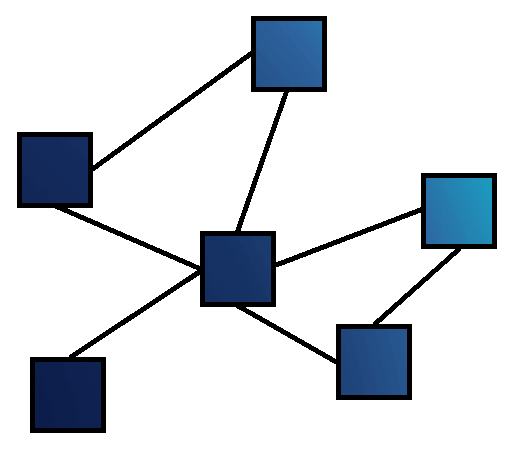
\includegraphics[scale=0.3]{{include/figuras/ModeloEnRed.png}}
    \caption{Modelo de red}
    \label{fig:bd_red}
\end{figure}

Al registro central se tiene acceso desde los otros cinco y desde él, puede accederse a otros cinco registros. En este modelo pueden definirse dependencias, de forma que si accedes al registro superior necesitas pasar por el central para poder alcanzar el registro de la derecha, como puede verse en la figura \ref{fig:bd_red}. Hoy en día este modelo de bases de datos se suele utilizar en algunos supercomputadores. Algunos de los modelos más conocidos son el UDS de Siemens y el DMS de Sperry Univac.

\subsubsection{Bases de Datos Relacionales}

Es el modelo más utilizado en la actualidad y es considerado como el estándar de la industria. Normalmente utiliza el lenguaje SQL y se trata de un modelo basado en tablas. Para definir las relaciones se utiliza álgebra relacional y gracias a esta se puede hallar la información de las diferentes relaciones como se puede ver en la figura \ref{fig:bd_relacional}.

\begin{figure}[h]
    \centering
    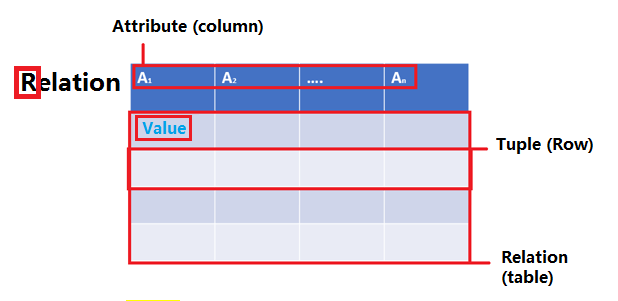
\includegraphics[scale=0.5]{{include/figuras/Relacional.png}}
    \caption{Modelo relacional}
    \label{fig:bd_relacional}
\end{figure}

El modelo relacional funciona mediante tablas independientes que determinan la organización de los datos y sus conexiones. Para poder identificar sin problema un registro es necesario establecer una \textbf{clave primaria}, que habitualmente se trata del primer atributo y no se puede modificar.

\subsubsection{Modelo de Base de Datos Orientado a Objetos}

Surgen a finales de 1980 y a día de hoy han tenido una aplicación muy minoritaria. Este tipo de bases de datos suelen utilizarse en plataformas de lenguajes Java y .NET. La más conocida es \textit{db4o} y destaca por su bajo consumo de memoria. Utilizan un lenguaje OQL, muy parecido a SQL.

\begin{figure}[h]
    \centering
    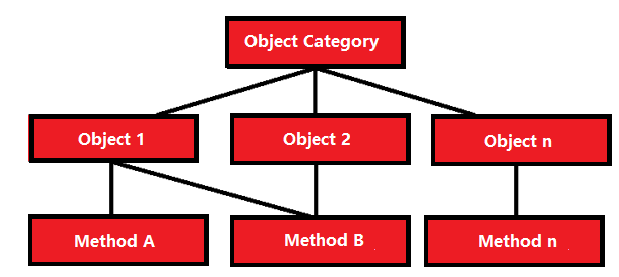
\includegraphics[scale=0.4]{{include/figuras/Objetos.png}}
    \caption{Modelo orientado a objetos}
    \label{fig:bd_objetos}
\end{figure}

En este modelo los datos se almacenan en objetos además de las funciones y los atributos que los definen (figura \ref{fig:bd_objetos}). Los objetos pueden ser complejos y estar formados por múltiples tipos de datos; se identifican por un identificador de objeto único y se agrupan en clases al igual que en lenguaje de programación orientado a objetos, creando una jerarquía de clases.

\subsubsection{Modelo de Base de Datos Orientado a Documentos}

En este modelo, la unidad mínima de almacenamiento de datos es el documento pero no se deben confundir con los documentos que se generan mediante un procesador de texto. En estos documentos los datos se almacenan como \textbf{pares claves-valor} tal y como se muestra en la figura \ref{fig:bd_documentos}, como no tienen una definición, los documentos que forman este tipo de bases de datos son muy diferentes entre sí. Cada documento es una unidad cerrada entre sí y establecer relaciones entre documentos no es una tarea sencilla, aunque por otro lado, en este tipo de bases de datos no es necesario establece relaciones.

\begin{figure}[H]
    \centering
    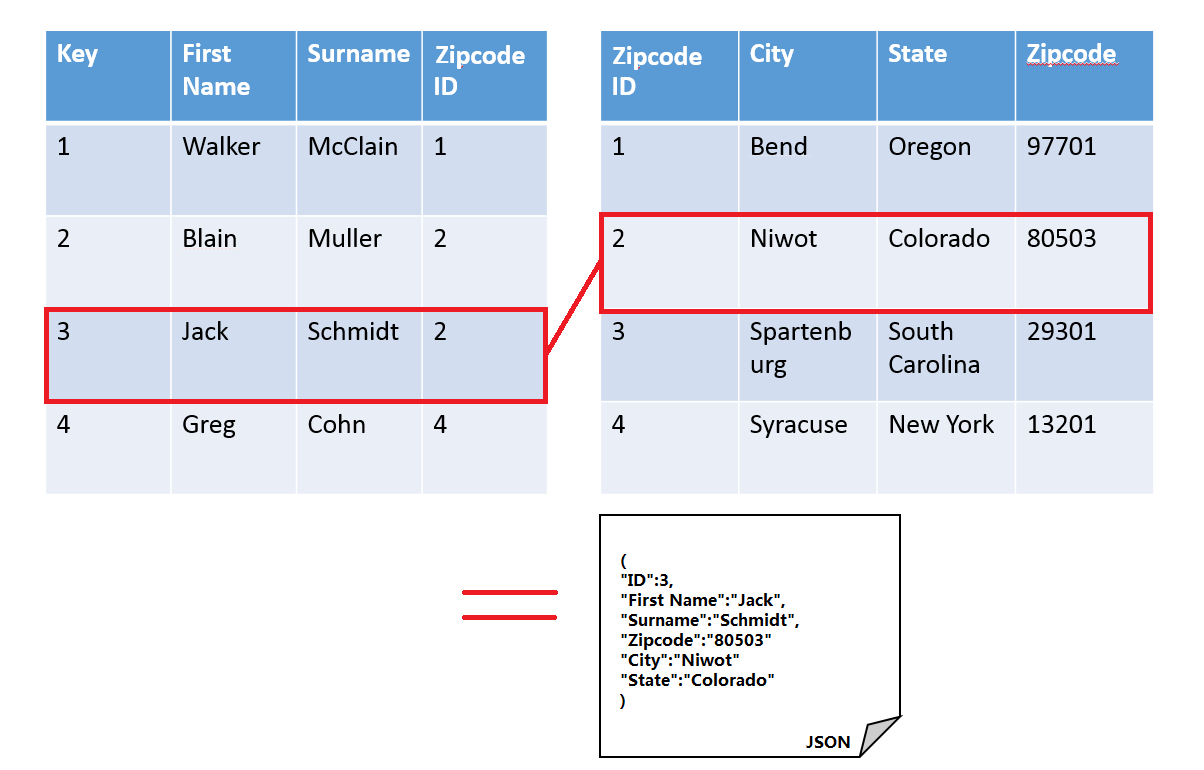
\includegraphics[scale=0.25]{{include/figuras/OrientadaDocumentos.png}}
    \caption{Modelo orientado a documentos}
    \label{fig:bd_documentos}
\end{figure}

La idea fundamental de este tipo de modelos es que los datos que tienen relación se guardan en un mismo documento, esto provoca que el número de consultas a la base de datos sea mucho menor que en una base de datos relacional. Son muy útiles para aplicaciones web debido a que puede almacenarse formularios HTML. Con el avance de la web 2.0 estas bases de datos aumentaron exponencialmente su popularidad y son utilizadas hoy en día por plataformas como Google, Facebook, Twitter, Amazon, etc.


\section{API REST}

\subsection{Historia de las API REST}

En la década de los 90, la gran mayoría de desarrolladores trabajaban con el protocolo \textit{SOAP} (abreviatura en inglés de Simple Object Access Protocol). Este protocolo consiste en el envío de datos mediante documentos escritos en lenguaje XML de forma manual, con una llamada RCP en el elemento \textit{body} y además era necesario especificar el endpoint. Esto lo convertía en una herramienta compleja de utilizar, construir y depurar. En ese momento no existía ninguna directriz o estándar sobre como diseñar y construir una API, sólo se buscaba la flexibilidad en el uso de la API.

En el año 2000, Roy Fieldind desarrolló en su tésis doctoral la manera mediante la cual dos servidores cualesquiera del mundo pudiesen establecer una comunicación entre sí. Para ello creó unos principios básicos, propiedades y restricciones que hoy en día se conocen como REST (es la abreviatura de Representational State Transfer). 

La empresa Salesforce fue la primera empresa en vender una API como una porción de un paquete de software en el año 2000, pero fueron muy pocos los desarrolladores que consiguieron aprovechar la API XML que venía además con un manual de uso de 400 páginas. 

Ebay viendo lo que Salesforce trataba de crear, decide construir una API accesible y de sencilla utilización y brinda acceso a sus socios además de equiparla con una documentación online exhaustiva. De esta manera, Ebay consiguió expandir su negocio fuera de su web Ebay.com a cualquier página capaz de acceder a su API. Debido a que la implementación seguía el estándar RESTful, muchos sitios web se apresuraron a aprovechar la oportunidad de expansión y de esta forma ampliar la oferta de productos a sus clientes. Amazon siguió rapidamente los pasos de Ebay, lo que propició que las plataformas web empezaran a cuantificar el valor de su código y no sólo el valor del producto que se pretendía vender. 

En 2004, Flickr lanza su propia API REST coincidiendo con el auge de las redes sociales. convirtiéndose rápidamente en una plataforma líder en la utilización de imágenes y permitiendo que se pudiese compartir e incrustar imágenes de forma sencilla en sitios web y feeds de redes sociales. Facebook se lanzó ese mismo año y Twitter en 2006, en un cominezo, ambas plataformas tenían sus APIs de forma interna lo que provocó que muchos desarrolladores utilizaron técnicas de scraping \footnote{Scraping: serie de técnicas empleadas para la obtención de datos en sitios web} y crearon sus propias API, al ser un cúmulo de métodos sin seguir un mismo diseño, se les conocía como API Frankestein. Esto provocó que ambos sitios lanzaran sus propias API oficiales en 2006.

En 2006, Amazon Web Services (AWS) comenzó a lanzar la nube. Esto permitía a los desarrolladores acceder a una cantidad enorme de datos a través de la API REST AWS. La implementación de APIs se ha multiplicado por más de 50 desde el año 2006 tal y como se puede ver en la figura \ref{fig:api}.

\begin{figure}[H]
    \centering
    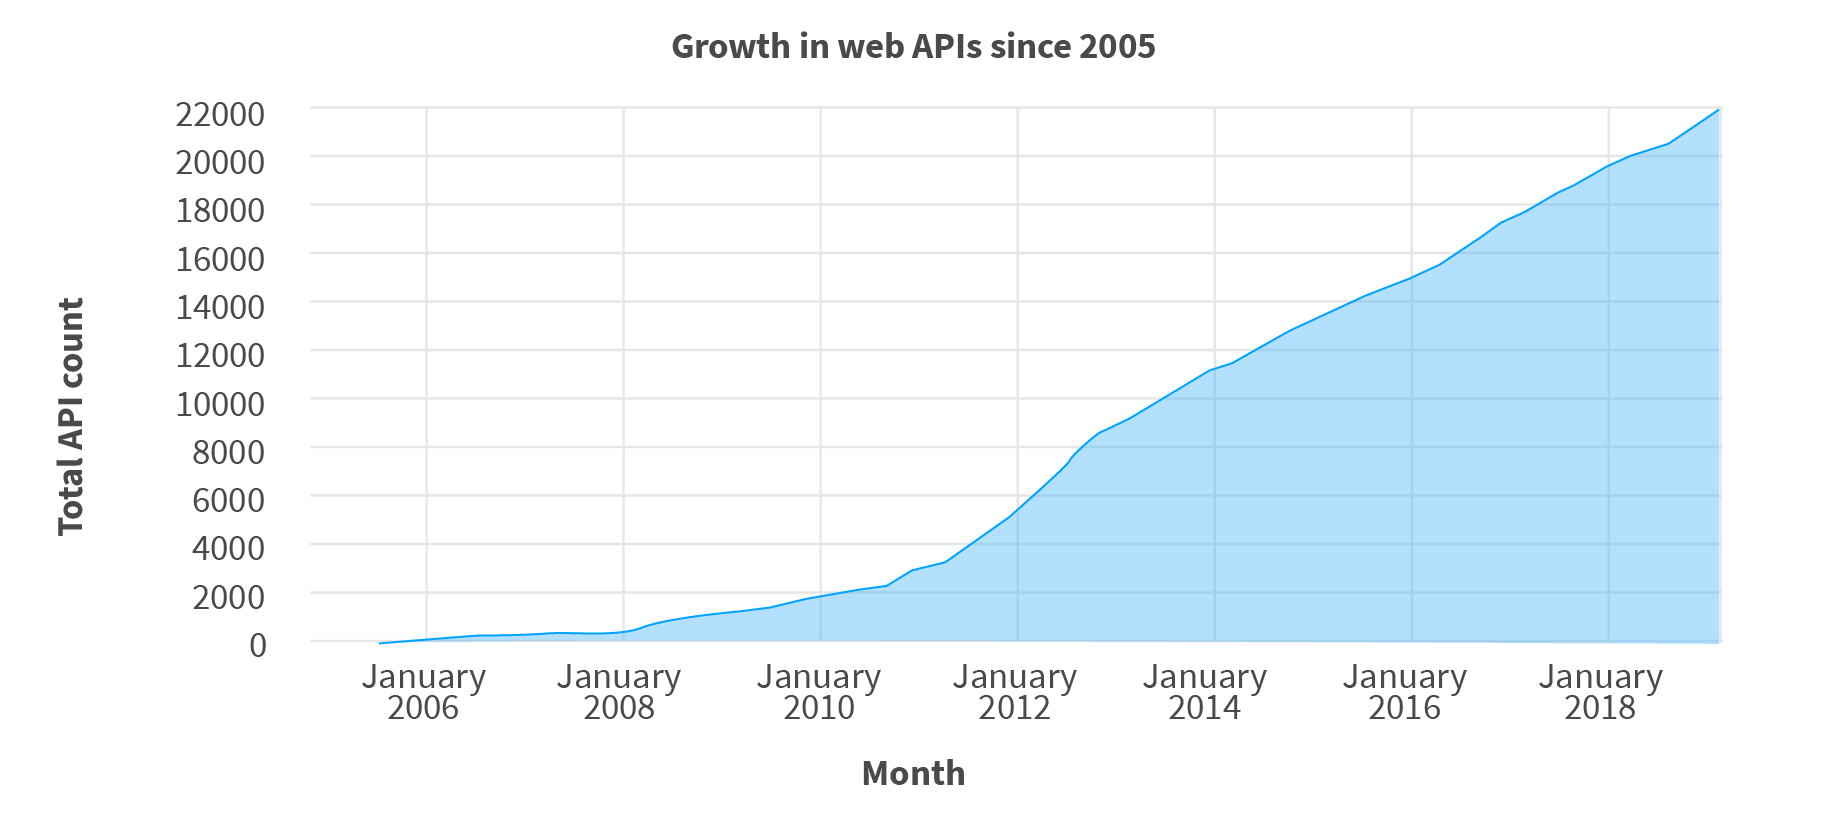
\includegraphics[width=\textwidth]{{include/figuras/API.png}}
    \caption{Crecimiento API Web desde 2005}
    \label{fig:api}
\end{figure}


Las APIs son las columnas de cualquier modelo de negocio y muchas veces se convierten directamente en el producto a vender por empresas de desarrollo de software. Gracias a la evolución de las API ya no es necesario tener equipos grandes de trabajo, cualquier desarrollador capaz de obtener una clave e interprete la documentación puede integrar funcionalidades de ese servicio en su software.

\subsection{Características principales}

Una API REST siempre utiliza los métodos implementados dentro del protocolo HTTP, son conocidos como verbos HTTP aunque también existe algún sustantivo. Cada uno de ellos tiene una llamada diferente aunque existen ciertas características compartidas. 

Los métodos de petición existentes son:

\begin{itemize}
    \item GET: solicita la representación del recurso especificado. Sólo recupera datos.
    \item HEAD: tiene el mismo comportamiento que la petición GET aunque sin recuperar el cuerpo de la respuesta.
    \item POST: con este método se envía información a un recurso específico.
    \item PUT: reemplaza todas las representaciones del recurso de destino con la información introducida en la petición.
    \item DELETE: elimina un recurso específico.
    \item CONNECT: establece una conexión hasta el servidor identificado en el recurso.
    \item OPTIONS: en él se describen las opciones de comunicación para el recurso de destino.
    \item TRACE: realiza una prueba de bucle de loop-back a lo largo de la ruta. 
    \item PATCH: se usa para realizar modificaciones parciales a un recurso.
\end{itemize}

Dentro de estas funciones las más utilizadas son POST, PUT, GET y DELETE. Cualquier API tiene que tener una serie de características comunes que se detallan a continuación:

\begin{itemize}
    \item Sin estado: cada petición HTTP contiene por sí sola la información necesaria para ejecutarse lo que permite que ni el servidor ni el cliente tengan que recordar ningún estado previo.
    \item Objetos manipulados con URI: una URI es un identificador único de cada recurso. Esto hace que sea más sencillo acceder a la información para modificarla o eliminarla.
    \item Interfaz uniforme: esto significa que siempre se utilizan los \textit{verbos HTTP} y siempre se utilizan las URIs de los recursos. Como resultado siempre se obtendrá una respuesta HTTP con un código de estado y un body.
    \item Sistema de capas: tiene una estructura jerárquica entre todos sus componentes y cada capa tiene una funcionalidad propia dentro del sistema REST. 
    \item Uso de hipermedios: los hipermedios permiten al usuario navegar entre objetos mediante enlaces HTML. En un API es la capacidad de una interfaz de dar al cliente y al servidor los enlaces necesarios para realizar acciones sobre datos.
\end{itemize}

\subsection{Ventajas de desarrollo con API REST}

La implementación de un API REST tiene múltiples ventajas, la más destacable de ellas es que se trata de un medio independiente a lenguajes de programación o plataformas de desarrollo, debido a que puede adaptarse a cualquier medio en el que se esté desarrollando, lo que proporciona una gran libertad. El único requisito indispensable es que se realicen las peticiones y las respuestas en XML o JSON. 

Al tratarse de un protocolo que separa totalmente al cliente y al servidor nos brinda una manera sencilla de exportar los proyectos a otros entornos y proporciona una gran escalabilidad. Además la separación nos permite tener el frontend y el backend desplegado en distintos servidores, dando a los desarrollos una gran flexibilidad a la hora de trabajar.


\subsection{API más populares}
